%!TEX root = ../crimson_throne_book_main.tex
% 2016-06-18
The sun has just set over the horizon when Quint and his friends return to the Gray district to prepare for the raid on the temple of Asmodeus. They decide to keep up the ruse of being Asmodean agents from Cheliax, sent here to put an end to the excesses of Archbisshop Ornher Reebs. As they make their way south, they encounter a Gray Maiden patrol. The officer asks them what they are still doing out, so they pretend to have been celebrating the queen's announcements. They lost track of time, but now they are on their way home. The soldiers buy their story and let them pass.\\

The party heads straight for the rebel base and informs the rebel leaders of what they have learned. They plan on invading the temple of Asmodeus tonight, but they have come here to get ready. Vencarlo offers to join the young men and Illrem offers them the use of his arsenal, from which they can get some helmets to cover their faces. Next the heroes pay a visit to Keppira d'Bear in the temple of Pharasma. The high priestess has a number of spells prepared that can help the companions in their quest against Reebs and his devils, but she does not dare enter the temple of Asmodeus with them out of fear of blowing her cover: although Pharasma supports the rebellion in secret, the church is trying to uphold a neutral position in public. She prepares a {\itshape heroes' feast} and sends one of her men to the Marble Dome opera house, to get a number of Asmodean theater outfits. Cloaked in tabards, capes and holy symbols of the Lord of Hell, the party returns to the old courthouse, just outside of the star-shaped temple of Asmodeus. This is as far as Keppira d'Bear will go. She casts other buffs on the party:  {\itshape greater magic weapon} on Balian's holy greatsword,  {\itshape magic vestment} ,  {\itshape protection from evil} and  {\itshape true seeing} on Quint,  {\itshape air walk} and  {\itshape align weapon} on Puk and  {\itshape magic circle versus evil} on Sjo. In the dead of night the party makes for the temple doors again. The Gray Maidens at the door let the 'inquisitor' and his bodyguards pass, as they were ordered to do by Tyresha. The church itself is abandoned, but Tyresha has put up a torch next to the door to the basement, showing the 'inquisitor' the way down. As they descend the stairs, the heroes pick up a sacrificial chant. Peeping around the corner, Puk sees a horrible scene.\hyperref[fig:Bloody-sacrifice-for-Asmodeus-616078986]{ A girl is being bled dry on a stone slab. } Her blood flows into an enormous pool, in which several amorphous shapes with half-formed limbs and dripping tumorous faces mill about, mixing the sanguine fluid with their own blood. These hideous lemure devils are the lowliest of the low in the ranks of hell, but even their inferior life energy contains the taint of the infernal. \hyperref[fig:Bloody-sacrifice-for-Asmodeus-2-616080218]{ Two Asmodean acolytes are actually performing the ritual } under the supervision of four Erinyes devils. \hyperref[fig:Asmodean-catacombs-blood-sarcifices-616082201]{ Two Gray Maidens complete the picture. } Quint sweeps into the room, taking up his role as inquisitor once again. He forbids the ritual, as it goes against the rules of this city. He wants to single out Ornher Reebs, but he notices the archbishop of Asmodeus is not here. \\

\begin{figure}[h]
	\centering
	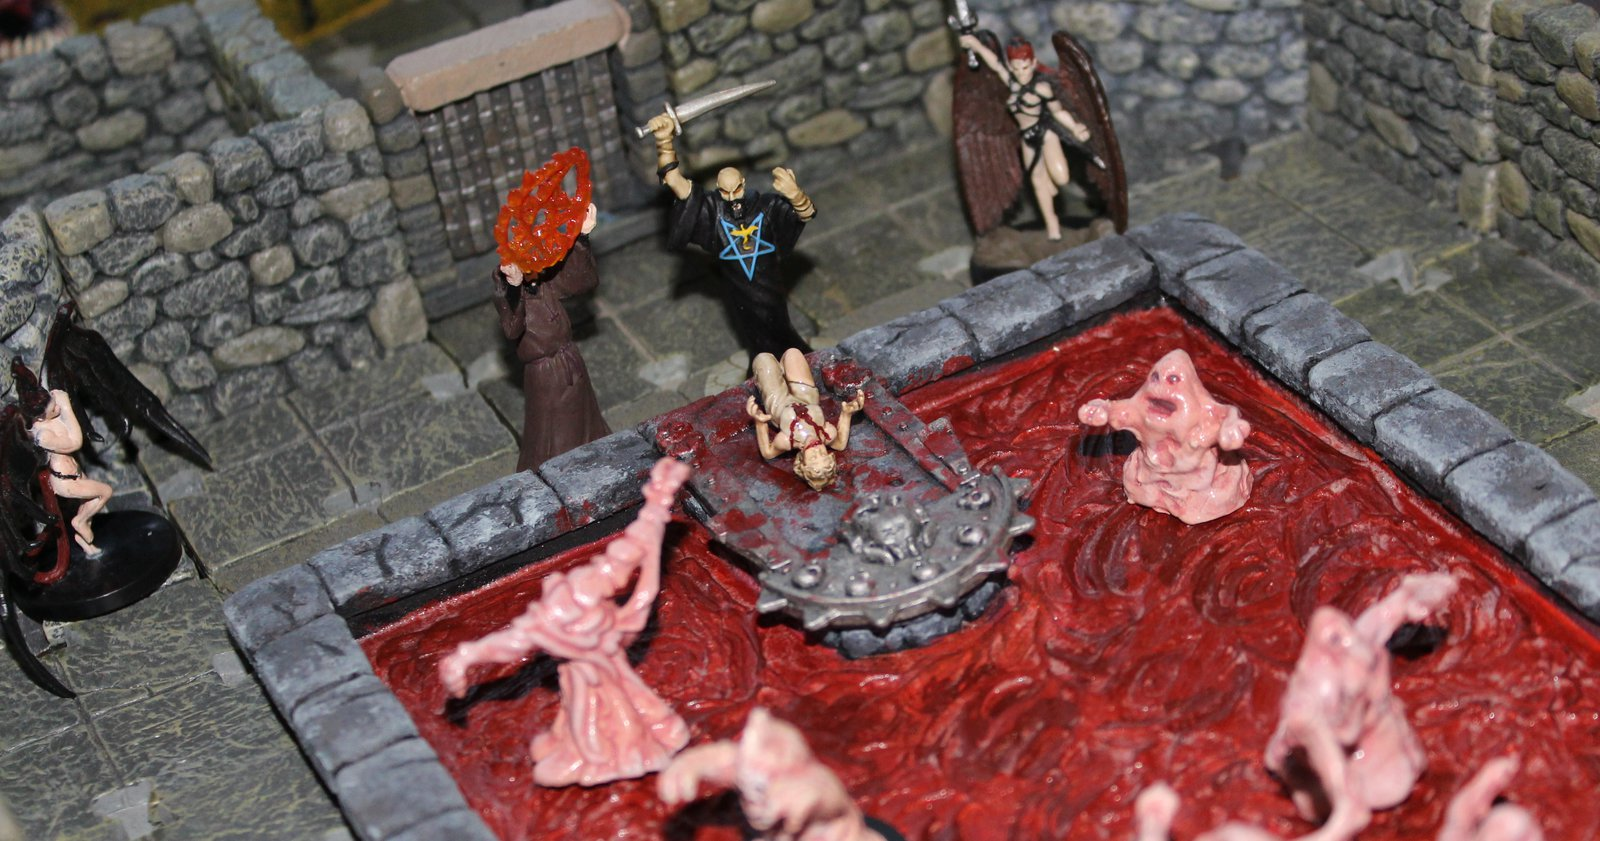
\includegraphics[width=0.4\textwidth]{images/Bloody-sacrifice-for-Asmodeus-616078986_mod.jpg}
	\caption{Bloody sacrifice for Asmodeus}
	\label{fig:Bloody-sacrifice-for-Asmodeus-616078986}
\end{figure}

\begin{figure}[h]
	\centering
	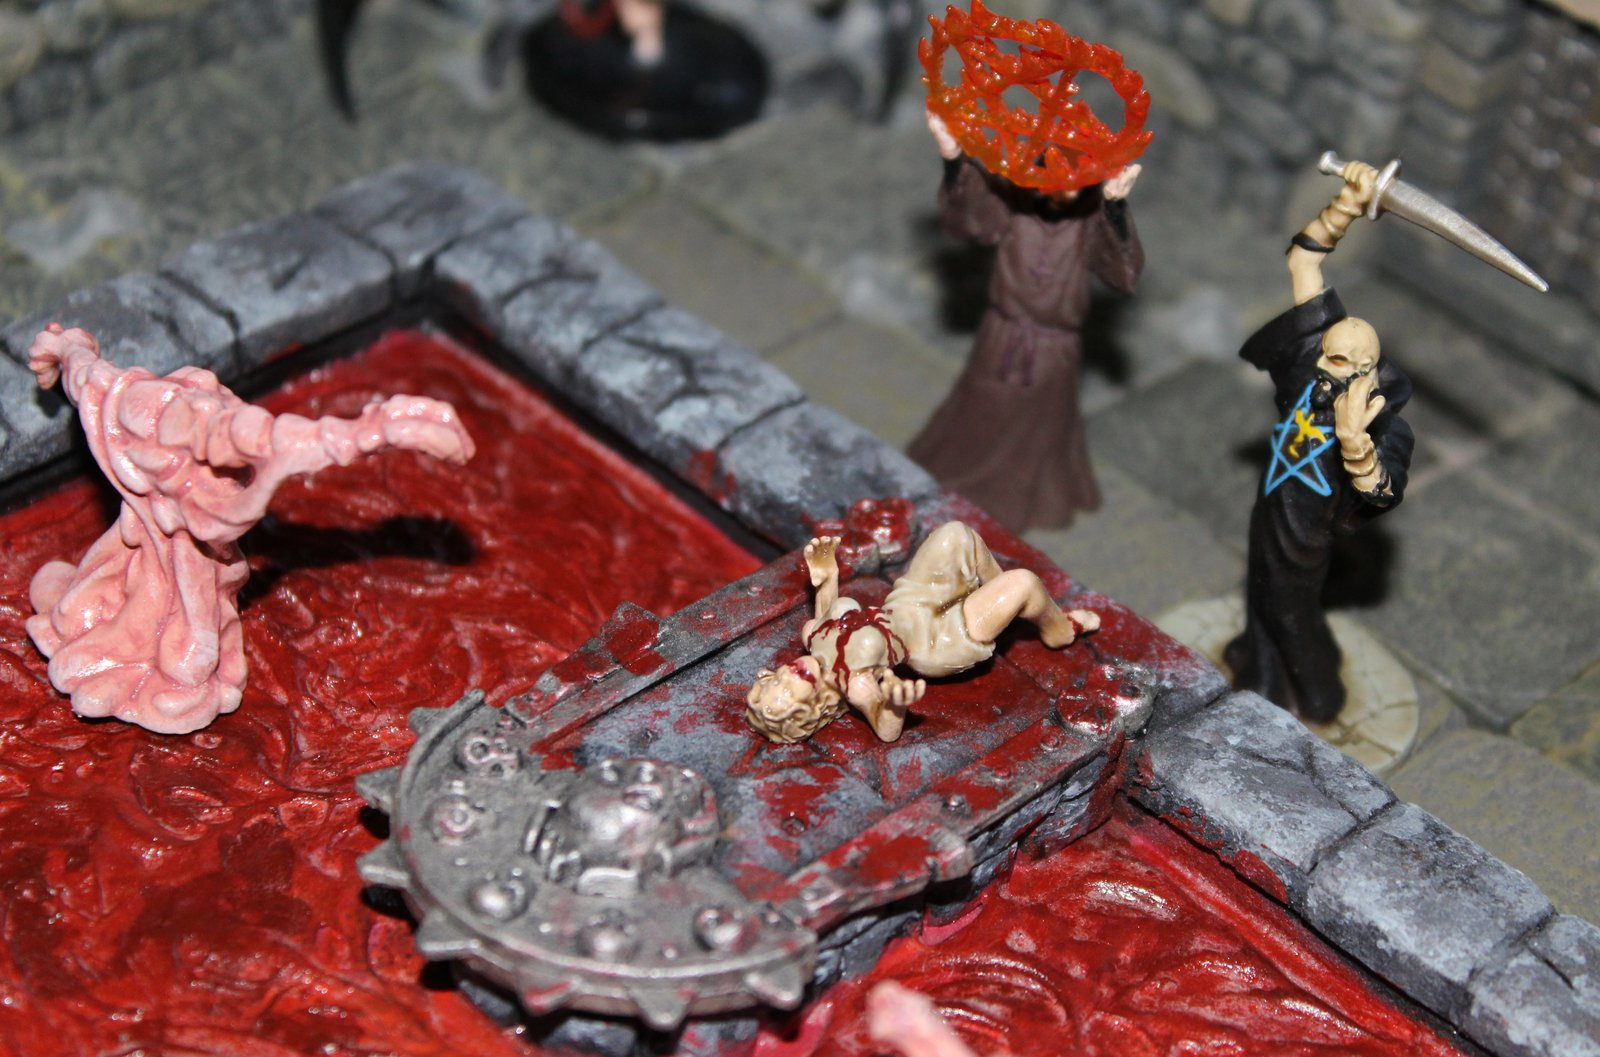
\includegraphics[width=0.4\textwidth]{images/Bloody-sacrifice-for-Asmodeus-2-616080218_mod.jpg}
	\caption{Bloody sacrifice for Asmodeus 2}
	\label{fig:Bloody-sacrifice-for-Asmodeus-2-616080218}
\end{figure}

\begin{figure}[h]
	\centering
	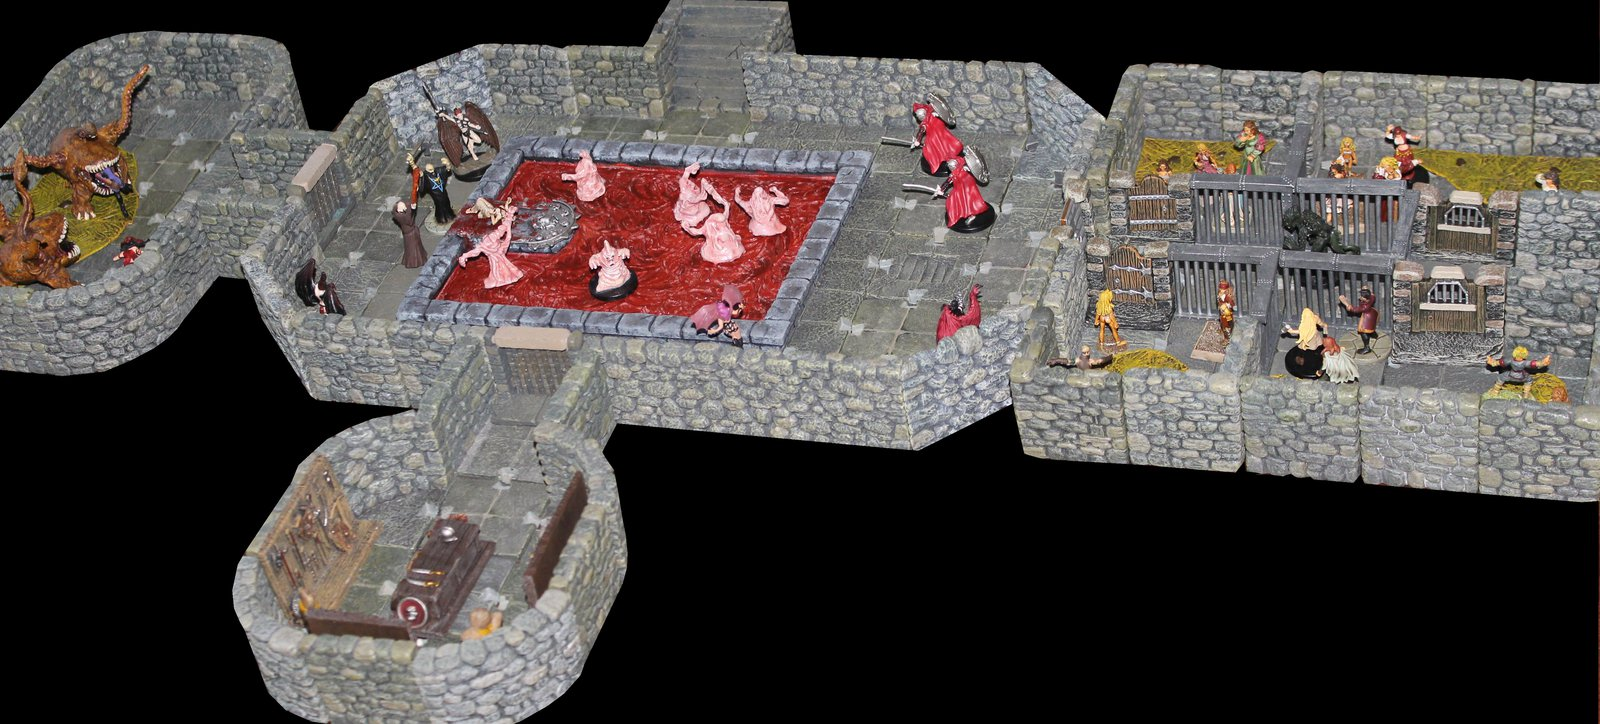
\includegraphics[width=0.4\textwidth]{images/Asmodean-catacombs-blood-sarcifices-616082201_mod.jpg}
	\caption{Asmodean catacombs blood sarcifices}
	\label{fig:Asmodean-catacombs-blood-sarcifices-616082201}
\end{figure}

The acolytes and even the Gray Maidens are taken aback by this sudden incursion, but the Erinyes are not fazed and open the fight. One of them casts {\itshape fear} on Balian, but the buffs on the ranger aid him in shaking off the spell. A second Erinyes throws  {\itshape unholy blight} on the party, while a third wraps her entangling rope around Sjo. The fourth charges Quint from the left with her longsword. The bard ducks under the blade and mumbles the words of  {\itshape good hope} to further strengthen his friends. He also starts a  {\itshape satire} to throw his enemies off balance. Vencarlo, Puk and Spyder jump to Quint's aid and engage the Erinyes, Balian wards off the Gray Maidens on the other side. One of them challenges him, but her swing misses him by an inch. Sjo tries to maintain his position in the center and boosts his companions with  {\itshape blessing of fervor} . Through his  {\itshape shield other} he also takes half of Balian's damage. The Gray Maidens, obviously blood clones, still prove tough opponents, but they fall short against the well-prepared and thoroughly buffed ranger. They manage to give him some nasty cuts, but a  {\itshape fireball} and a critical sword swing later, one of them explodes in a spray of blood. Without her ally, the second maiden is severely at a disadvantage. In the meantime Quint has cast {\itshape haste} and feinted one of the Erinyes, giving his friends there the opportunity to cut her down. From across the pool two Erinyes are still hurting the party with arrows and  {\itshape unholy blights} . One moment later a door to their right opens and the barbed devil joins the fray \hyperref[fig:Gray-Maiden-recruits-of-sacrifices-616081293]{ from what looks to be a prison block filled with young girls. } Another powerful opponent is not exactly good news, but Quint is happy to see that there is still a fair number of 'recruits' alive, making this rescue mission even more valuable. The barbed devil hurts the party with an alternative spell, that does not target 'good' characters, but rather 'chaotic' ones:  {\itshape order's wrath} . Balian takes another hit before he can take out the second Gray Maiden and turns to face the barbed jailor. Sjo is hurting from his own wounds as well as from half of Balian's, and gives himself some much required healing. Another  {\itshape unholy blight} on Vencarlo and Puk in the left flank takes down the halfling and leaves the sword master barely on his feet. With his flashing rapier Vencarlo kills a second Erinyes and stumbles back to Sjo' side. \\

\begin{figure}[h]
	\centering
	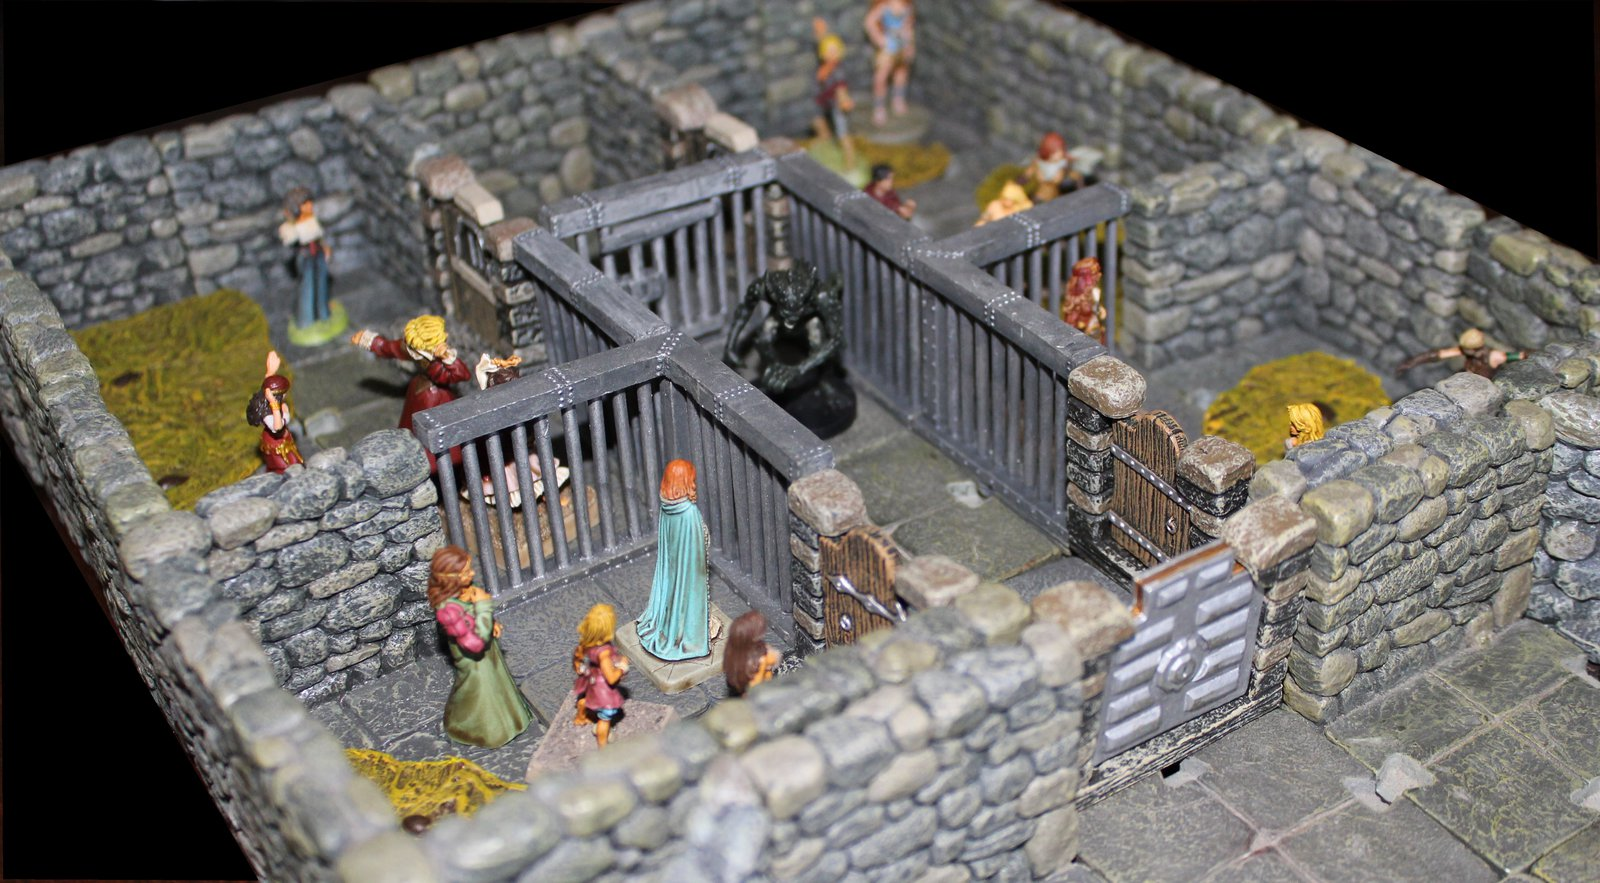
\includegraphics[width=0.4\textwidth]{images/Gray-Maiden-recruits-of-sacrifices-616081293_mod.jpg}
	\caption{Gray Maiden recruits or sacrifices?}
	\label{fig:Gray-Maiden-recruits-of-sacrifices-616081293}
\end{figure}

The two Asmodean acolytes have not contributed anything to the fight so far, clearly being outmatched. One of them desperately prays to his god for aid as he stabs the sacrifice on the stone slab one more time, but the girl was already gone. The other one opens the left door, freeing the two wild otyughs who are there to dispose of the cadavers. One of the aberrations rewards the stupid priest by eating him alive, while the other monster turns on Sjo, who has is trying to patch up Vencarlo and Puk. The otuygh's tentacle grabs hold of the healer, but now the monster opens itself up to sneak attacks by Puk and Vencarlo, cutting its life short.\\

On the other side of the room Balian withstand a {\itshape hold person} from the barbed devil and seriously hurts the infernal creature with three heavy blows. This being has probably lived a thousand lifetimes and knows when it is time to retreat, so it steps back and  {\itshape teleports} away. The two remaining Erinyes, who are now facing Puk and Balian, see how their more powerful ally has chosen to flee the scene and do the same. Quint walks up to the one acolyte who is still left and shouts at him: {\itshape``Where is Reebs?}'' Totally intimidated the priest stumbles back: {\itshape``Below us, in the cellar!}'' Then Spyder jumps at him and ends his miserable life. Puk and Balian take care of the second otuygh, while Quint decides to close the door to the cell block. He desperately wants to tell the caged girls they are free, but cannot spare the time as he wants his buffs to remain intact to confront Reebs. The party heals up and prepares to descend the stairs to deliver justice to Reebs. \section{Level up: level 10}


